\svnidlong
{$HeadURL$}
{$LastChangedDate$}
{$LastChangedRevision$}
{$LastChangedBy$}
\svnid{$Id: $}


%%%%%%%%%%%%%%%%%%%%%%%%%%%%%%%%%%%%%%%%%%%%
%\section*{EFT Validity and Truncation Summary}
%%%%%%%%%%%%%%%%%%%%%%%%%%%%%%%%%%%%%%%%%%%%

Effective Field Theories (EFTs) are an extremely useful
framework for interpreting DM searches at the LHC.
Given our current lack of knowledge about the nature of a DM particle and
its interactions, a model independent interpretation of the collider bounds
appears mandatory.  This approach should be complemented with
an interpretation within a choice of simplified models.
However, these models cannot exhaust the set of possible completions of
an effective Lagrangian.
EFTs must be used with caution at colliders, where the energy
scale of the interaction can be above the point where the EFT
approximation is valid.

To illustrate the problem, consider an effective interaction
$$ (\bar\psi\psi)(\bar\chiDM\chiDM) {g\over \Lambda^2}$$
that couples SM and DM fields.   The strength of this interaction can
be parametrized by $f={g\over \Lambda^2}$.
A monojet signature can be generated
by applying perturbation theory in the QCD coupling (assuming $\phi$\Todo{right symbol?} is
a quark, for example).
An experimental search will place a limit on $f$.   
For a fixed $f$, a small value of $g$ will require
a small value of $\Lambda$.   The EFT approximation breaks down
if $Q>\Lambda$, where $Q$ is a typical hard scale of the process.
One reasonable choice is $\Qtr^2=p(\bar\chiDM\chiDM)^2$, i.e.
the momentum flow through
the \schannel.  
On the other hand, large $\Lambda$
implies large $g$, raising the question if perturbation theory
is even applicable.     

Here we summarize some methods that can be used to ensure the validity of the EFT approximation. These methods are described in detail in Refs.~\cite{Busoni:2013lha,Busoni:2014sya,Busoni:2014haa,Aad:2015zva,Racco:2015dxa}. We then propose a recommendation for the presentation of EFT results for Run-2 LHC benchmarks.

%%%%%%%%%%%%%%%%%%%%%%%%%%%%%%%%%%%%%%%%%%%%
\section{\texorpdfstring{Outline of the procedure described in Refs.~\cite{Busoni:2014sya,Aad:2015zva}}{Outline of the procedure described in Refs.}}
\label{sec:TruncationWithQTr}
%%%%%%%%%%%%%%%%%%%%%%%%%%%%%%%%%%%%%%%%%%%%

A standard approach has been to consider a simplified model and work backwards to determine the validity of the EFT approximation.
For a tree-level interaction between DM and the Standard Model (SM) via some mediator with mass \mMed, the EFT approximation corresponds to
expanding the propagator for the mediator
in powers of $\Qtr^2/\mMed^2$, truncating at lowest order, and combining the remaining parameters into a single parameter \Mstar (also called $\Lambda$ in the literature).
For an example scenario with a \Zprime-type mediator (leading to some combination of operators D5 to D8 in the EFT limit)
this corresponds to setting
%
\be
\frac{\gDM \gq}{Q_{\rm tr}^2-M^2}=-\frac{\gDM \gq}{M^2}\left(1+\frac{Q^2_{\rm tr}}{M^2}+ \mathcal{O} \left(\frac{Q^4_{\rm tr}}{M^4}\right)\right) \simeq -\frac{1}{{\Mstar}^2},
\ee
%
where $\Qtr$ is the momentum carried by the mediator, and $\gDM$, $\gq$ are the DM-mediator and quark-mediator couplings respectively. Similar expressions exist for other operators. Clearly the condition that must be satisfied for this approximation to be valid is that $\Qtr^2 < M^2 = \gDM \gq {\Mstar}^2$. 
In this framework, there are clearly three regions to consider:
\begin{itemize}
\item $\Qtr^2 \sim M^2$, in which case the EFT misses a resonant enhancement, and it is conservative to ignore this enhancement;
\item $\Qtr^2 \ll M^2$, in which case the EFT is valid; and
\item $\Qtr^2 \gg M^2$, in which case the signal cross section should fall according to a power of $\Qtr^{-1}$ instead of $M^{-1}$.   This is the problematic kinematic region.
\end{itemize}

We can use the condition $\Qtr^2 < M^2 = \gDM \gq {\Mstar}^2$ to restrict the
kinematics of the signal
and enforce the validity of the EFT approximation (after the imposition of the event selection of the analysis).  This truncated signal can then be used to derive the new, truncated limit on $\Mstar$ as a function of $(\mDM, \gDM \gq)$.
 
For the example D5-like operator, $\sigma \propto {\Mstar}^{-4}$, and so there is a simple rule for converting a rescaled cross section into a rescaled constraint on ${\Mstar}$ if the original limit is based on a simple cut-and-count procedure. Defining $\sigma_{\rm EFT}^{\rm cut}$ as the cross section truncated such that all events pass the condition $\sqrt{\gDM \gq} \Mstar^{\rm rescaled} > \Qtr$, we have
%
\be
\Mstar^{\rm rescaled} = \left(\frac{\sigma_{\rm EFT}}{\sigma_{\rm EFT}^{\rm cut}}\right)^{1/4} \Mstar^{\rm original},
\ee
%
which can be solved for $\Mstar^{\rm rescaled}$ via either iteration or a scan (note that $\Mstar^{\rm rescaled}$ appears on both the LHS and RHS of the equation). Similar relations exist for a given UV completion of each operator. The details and application of this procedure to ATLAS results can be found in Ref.~\cite{Aad:2015zva} for a range of operators. Since this method uses the physical couplings and energy scale $\Qtr$, it gives the strongest possible constraints in the EFT limit while remaining robust by ensuring the validity of the EFT approximation. 

If a search is not simply a counting experiment and exploits the shapes of kinematic distributions, the condition on the momentum transfer should be applied on the benchmarks using generator level information, by discarding events that are invalid. This provides the necessary rescaling of the cross section while keeping the information on the change in the kinematic distributions due to the removal of the invalid events. 

\clearpage

%%%%%%%%%%%%%%%%%%%%%%%%%%%%%%%%%%%%%%%%%%%%
\section{\texorpdfstring{Outline of the procedure described in Ref.~\cite{Racco:2015dxa}}{Outline of the procedure described in Refs.}}
\label{sec:TruncationWithSHat}
%%%%%%%%%%%%%%%%%%%%%%%%%%%%%%%%%%%%%%%%%%%%

In \cite{Racco:2015dxa} a procedure to extract model independent and consistent bounds within the EFT is described. This procedure can be applied to any effective Lagrangian describing the interactions between the DM and the SM, and provides limits that can be directly reinterpreted in any completion of the EFT.

The range of applicability of the EFT is defined by a mass scale \Mcut, a parameter which marks the upper limit of the range of energy scales at which the EFT can be used reliably, independently of the particular completion of the model. 
Regardless of the  details of the full theory, the energy scale probing the validity of the EFT is less than or equal to the center-of-mass energy $E_\text{cm}$, 
the total invariant mass of the hard final states of the reaction.
To be specific, consider the basic mono-jet process with kinematics
$p_1 + p_2 \to k + p_{\bar\chiDM\chiDM}$: $k$ is the momentum of the outgoing jet, whereas $p_{\bar\chiDM\chiDM}$ is the momentum of the $\bar\chiDM\chiDM$ pair and
$p_{\bar\chiDM\chiDM}=\Qtr$.  $E_\text{cm}^2 = (p_1+p_2)^2 > \Qtr^2$.
The condition ensuring the validity of the EFT is, by definition of \Mcut,
\begin{equation}
\label{Ecm<Mcut}
E_\text{cm}<M_\text{cut}\,.
\end{equation}
For example, in the specific case of a tree level mediation with a single mediator, \Mcut can be interpreted as the mass of that mediator.

There are then at least three free parameters describing an EFT:~ 
the DM mass $m_\text{DM}$, the scale $\Mstar$ of the interaction, and the cutoff scale \Mcut.

We can use the same technique as above to restrict the signal to the events for which $E_\text{cm}<M_\text{cut}$,  using only these events to derive the exclusion limits on $\Mstar$ as a function of  $(m_\text{DM},M_{\rm cut})$. 
%
We can also define an \textit{effective coupling strength} $\Mcut=\gstar \, \Mstar\,,$ where \gstar is a free parameter that substitutes the parameter \Mcut, and therefore derive exclusions on \Mstar as a function of $(\mDM,\gstar)$. This allows us to see how much of the theoretically allowed parameter space has been actually tested and how much is still unexplored; For example, in the \Zprime-type model considered above, \gstar is equal to $\sqrt{\gDM\gq}$.
%
The resulting plots are shown in \cite{Racco:2015dxa} for a particular effective operator. 

The advantage of this procedure is that the obtained bounds can be directly and easily recast in any  completion of the EFT, by computing the parameters \Mstar, \Mcut in the full model as functions of the parameters of the complete theory. On the other hand, the resulting limits will be weaker than those obtained using \Qtr and a specific UV completion.

\section{Comments on Unitarity Considerations}
\todo{Waiting for comments from J. Alcaraz}

\section{Recommendation for presentation of EFT results} %change this title
\label{sec:RecommendationEFTResults}

A full discussion of the presentation of collider results is left to 
work beyond this Forum, where ATLAS, CMS, the theory community
and the Direct and Indirect Detection communities are involved. 
In this report we recommend two strategies for the presentation of results
in terms of Effective Field Theories. We divide the EFT operators in two categories: 
those which can be mapped to one or more UV-complete simplified models, such as those
commonly used in LHC searches so far and detailed in~\cite{Goodman:2010ku}, and those
for which no UV completion is available, such as those outlined in Section~\ref{sec:EFT_models_with_direct_DM_boson_couplings}. Results for the first class
of operators can be recast using simplified models with high mediator masses, therefore removing
the need to explicitly simulate EFT events and provide experimental limits
for those operators. For the second class of models, a truncation procedure 
should be applied and the truncated results should be presented alongside 
the naive EFT results.

Three proposals for the treatment of EFT have been stated so far:
(1) truncate using \Qtr, (2) truncate and iterate using \Qtr, and
(3) truncate using \Ecm.   Another possibility is to
present the raw EFT results, but qualify that they might not be
valid.  Finally, one can quantify the validity of the EFT result
by presenting the sensitivity to \Reft, the fraction of events
that satisfy $\hat{s} > \Mcut ^2$, for example.

\section{Recommendation for contact interaction theories with simplified models available}

\begin{figure}
\centering
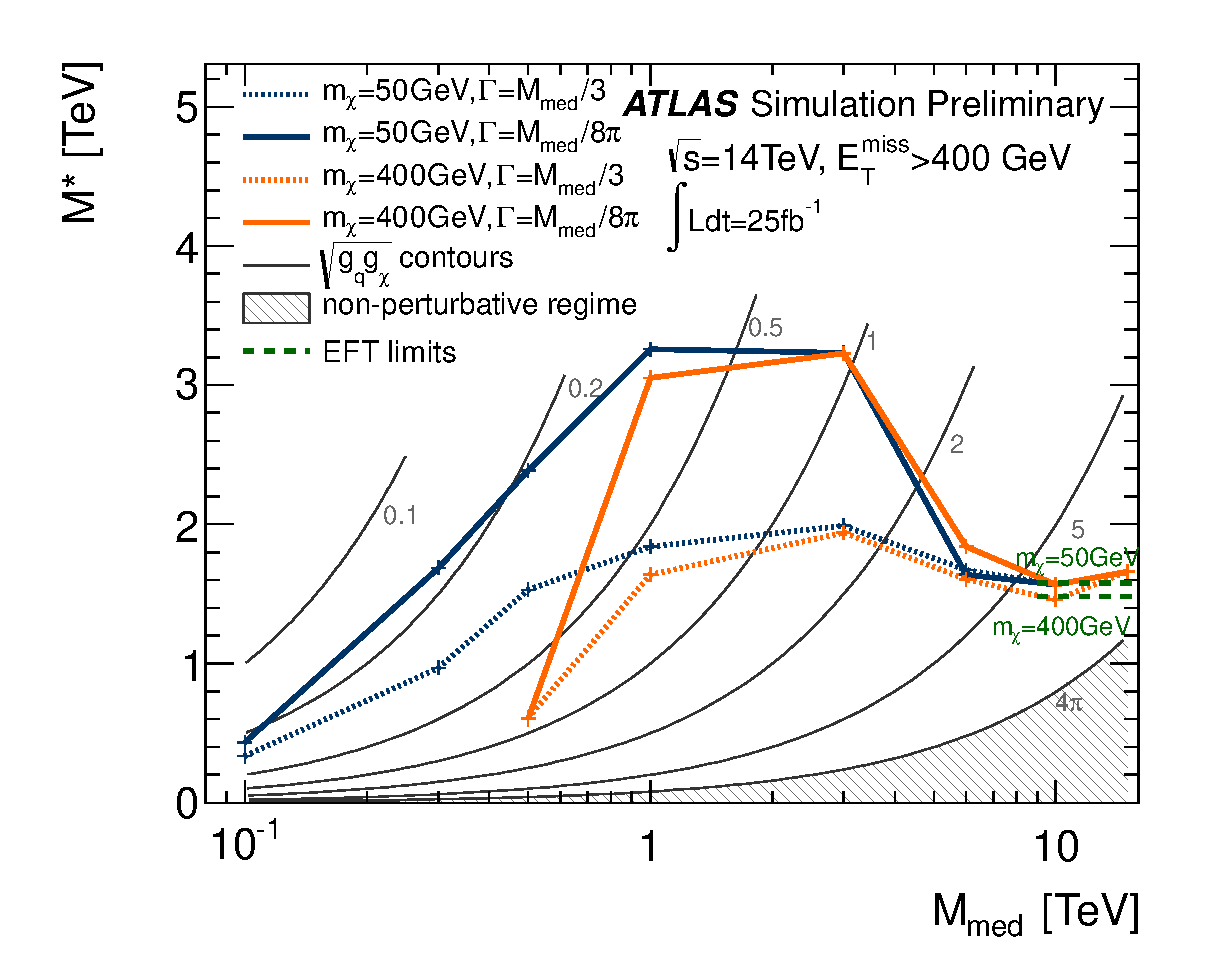
\includegraphics[width=0.9\textwidth]{figures/monojet/lambda_14TeV_SR1.eps}
\caption{Comparison of the 95\% CL lower limits on the scale of the interaction of a \Zprime-like simplified model at 14~\tev, in terms of the mediator mass. Corresponding limits from EFT models are shown on the same plot as green dashed lines to show equivalence between the two models for high mediator masses.
Taken from Ref.\,\cite{ATL-PHYS-PUB-2014-007}.}
\label{fig:monojet_MstarMmed}
\end{figure}

If a simplified model can be mapped to a given EFT, then the model's high-mediator-mass limit 
will converge to the EFT. This can be seen in Fig.~\ref{fig:monojet_MstarMmed}, where the limits on 
the scale of the interaction of a \Zprime-like simplified model are presented in terms of the mediator mass~\footnote{This plot only serves as exemplification of the convergence of the simplified model to a contact
	interaction operator: before this Report, ATLAS and CMS searches presented search results up to very high couplings and therefore high widths, potentially probing unphysical corners of phase space}. 
The limits at high mediator mass for this model are equivalent to those of the corresponding EFT benchmark. 
For this reason, experimental collaboration should deliver results for high-mass mediators instead of 
pure EFT results, and leave further reinterpretation to theorists.
\Todo{The extrapolation to other couplings and mediator masses can be
done using the \Qtr prescription for that model.}

We therefore recommend the addition of one point at very high mediator mass (5 \tev) to the scan, for each of the DM masses for the simplified models described in Section~\ref{subsec:MonojetLikeModels}. The truncation procedure in Section~\ref{sec:TruncationWithSHat} can be used to fine-tune the mediator mass to be simulated for this purpose. Studies are ongoing for $s-$channel vector mediators. 

%\Todo{Is this sufficient information for reinterpretation, or should we have instructions?}

\section{Recommendation for truncation of theories with no simplified models available}

Whenever a UV completion is not available, EFT results can still
be a source of useful information as 
described in Section~\ref{sub:validityEWContact}. 
However, we can only naively control the validity of the EFT operator.
Despite the fact that a propagator was introduced to motivate
the truncation procedure for \schannel models, the prescription
is only dependent upon the simplified model to derive the
energy scaling.   The simple fact remains that the effective
coupling of the operator -- $g/\Lambda^n$ -- should not allow
momentum flow $Q>\Lambda$ or $g>4\pi$.  Given our ignorance of
the actual kinematics, 
the truncation procedure suggested for this purpose
is the one described in Section~\ref{sec:TruncationWithSHat},
as it is independent from any UV completion details. 

Because there is no UV completion,
the parameter \Mcut can be treated more freely than
an explicit function of $g$ and $\Lambda$.
It makes sense to choose \Mcut such that we 
identify the transition region where the EFT stops being
a good description of UV complete 
theories. This can be done using the ratio \Reft, which is defined
as the fraction of events for which $s_{hat} > \Mcut^2$. 
For large values of \Mcut, no events are thrown away in the truncation 
procedure, and R=1. As \Mcut becomes smaller, eventually all events are thrown 
away in the truncation procedure, i.e. $\Reft=0$, and the EFT gives no 
exclusion limits for the chosen acceptance.  

We propose a rough scan over \Mcut, such that we find the values of \Mcut 
for which \Reft ranges from 0.1 to 1. The analysis can then perform a scan over 
several values of \Mcut \Todo{agree on how many?}, and show the truncated limit 
for each one of them alongside the naive limit corresponding to $\Reft=1$. 

%When \Reft=0, there is no limit. When \Reft reaches 1, the truncated limit 
%is identical to the original limit. (<== These last two sentences may be overkill. 
%Cut it if you think this is already clear)

